For the validation of the proposed feature augmented classifier, we create a dataset of 30 fruits and vegetables (see Table \ref{tab:veg_types}). We capture 10 RGB images for each type of fruit or vegetable. Each of these images are rotated 7 times to create new images, resulting in a total of 2400 RGB images for training.

\bgroup
\def\arraystretch{1.5}
\begin{table}[htbp]
	\caption{Types of Fruits and Vegetables Used for Creating the Dataset}
	\begin{center}
		\begin{tabular}{| >{\centering\arraybackslash}m{2cm} | >{\centering\arraybackslash}m{2cm} | >{\centering\arraybackslash}m{2cm} |}
			\hline
			Cabbage & White Turnip & \\
			\hline
			Tomato & Okra & \\
			\hline
			Orange Pepper & Eggplant & \\
			\hline
			Red Pepper & Squash Zucchini & \\
			\hline
			Jalapeno & Carrot & \\
			\hline
			Green Pepper & & \\
			\hline
			Beet & & \\
			\hline
			Daikon Lo Bok & & \\
			\hline
			Bok Choi & & \\
			\hline
			Brussel Sprout & & \\
			\hline
		\end{tabular}
		\label{tab:veg_types}
	\end{center}
\end{table}
\egroup

As Fig. \ref{fig:veg_rotations} shows, the 7 rotations are applied at increasing increments of 45\degree{} starting from the original. We do this to account for non-symmetric fruits and vegetables that are not axis aligned.

\bgroup
\def\arraystretch{1.5}
\begin{figure*}[tp]
	\begin{center}
		\begin{tabular}{c|ccccccc}
			Original & \multicolumn{7}{c}{Rotated} \\
			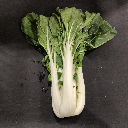
\includegraphics[scale=0.4]{./img/bokchoi_0.png} &
			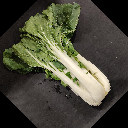
\includegraphics[scale=0.4]{./img/bokchoi_1.png} &
			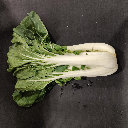
\includegraphics[scale=0.4]{./img/bokchoi_2.png} &
			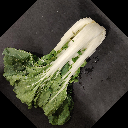
\includegraphics[scale=0.4]{./img/bokchoi_3.png} &
			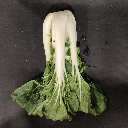
\includegraphics[scale=0.4]{./img/bokchoi_4.png} &
			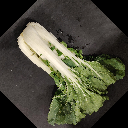
\includegraphics[scale=0.4]{./img/bokchoi_5.png} &
			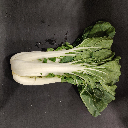
\includegraphics[scale=0.4]{./img/bokchoi_6.png} &
			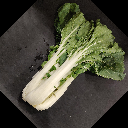
\includegraphics[scale=0.4]{./img/bokchoi_7.png} \\
			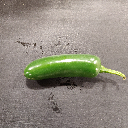
\includegraphics[scale=0.4]{./img/jalapeno_0.png} &
			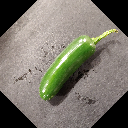
\includegraphics[scale=0.4]{./img/jalapeno_1.png} &
			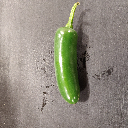
\includegraphics[scale=0.4]{./img/jalapeno_2.png} &
			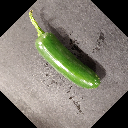
\includegraphics[scale=0.4]{./img/jalapeno_3.png} &
			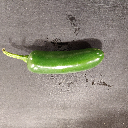
\includegraphics[scale=0.4]{./img/jalapeno_4.png} &
			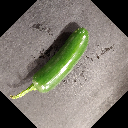
\includegraphics[scale=0.4]{./img/jalapeno_5.png} &
			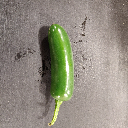
\includegraphics[scale=0.4]{./img/jalapeno_6.png} &
			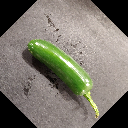
\includegraphics[scale=0.4]{./img/jalapeno_7.png} \\
			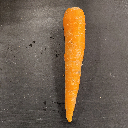
\includegraphics[scale=0.4]{./img/carrot_0.png} &
			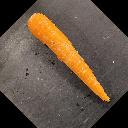
\includegraphics[scale=0.4]{./img/carrot_1.png} &
			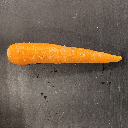
\includegraphics[scale=0.4]{./img/carrot_2.png} &
			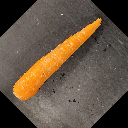
\includegraphics[scale=0.4]{./img/carrot_3.png} &
			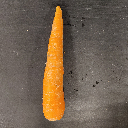
\includegraphics[scale=0.4]{./img/carrot_4.png} &
			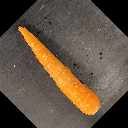
\includegraphics[scale=0.4]{./img/carrot_5.png} &
			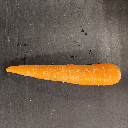
\includegraphics[scale=0.4]{./img/carrot_6.png} &
			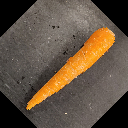
\includegraphics[scale=0.4]{./img/carrot_7.png} \\
			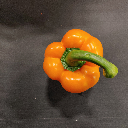
\includegraphics[scale=0.4]{./img/pepper_0.png} &
			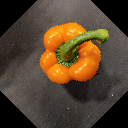
\includegraphics[scale=0.4]{./img/pepper_1.png} &
			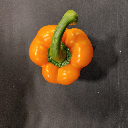
\includegraphics[scale=0.4]{./img/pepper_2.png} &
			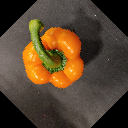
\includegraphics[scale=0.4]{./img/pepper_3.png} &
			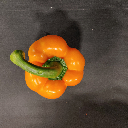
\includegraphics[scale=0.4]{./img/pepper_4.png} &
			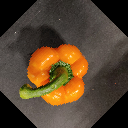
\includegraphics[scale=0.4]{./img/pepper_5.png} &
			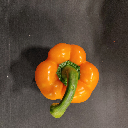
\includegraphics[scale=0.4]{./img/pepper_6.png} &
			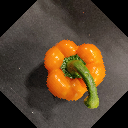
\includegraphics[scale=0.4]{./img/pepper_7.png} \\
		\end{tabular}
		\label{tab:veg_types}
	\end{center}
	\caption{Four sample images with their rotated counterparts.}
	\label{fig:veg_rotations}
\end{figure*}
\egroup